\chapter{Additional notes on convection-diffusion}

\section{Boundary layers in robust norm test functions and global/local test spaces}
\seclab{appendix:globalLocal}

In Section~\secref{sec:testNormSec}, we introduced the test norm
\[
\nor{v,\tau}_V^2 \coloneqq \alpha\nor{v}_{\L}^2 + \nor{\beta\grad v}_{\L}^2 + \epsilon \nor{\grad v}_{\L}^2 + {\min}\LRc{\frac{1}{\epsilon},\frac{1}{\LRb{K}}}\nor{\tau}_{\L}^2 + \nor{\div \tau}_{\L}^2
\]
where $\alpha \in [\epsilon,1]$ was selected in such a way that optimal test functions over a single element did not contain boundary layers\footnote{Boundary layers can appear in the cross-stream direction if $\alpha$ is not the same order as $\epsilon/h^2$, where $h$ is the element size.  This is explained in more detail in \cite{DPGrobustness2}} which are difficult to approximate using our enriched space.  

However, in \cite{globalLocalDPG}, it was shown that the global test space made up of the union of local test spaces contains the test subspace of weakly conforming test functions that are the result of solving for optimal test functions globally using a weakly conforming enriched space (which we refer to as the \textit{global test space}).  Furthermore, the field solutions for the DPG method are dependent only upon the properties of the global test space.  

In other words, the resolution of boundary layers that occur at element boundaries is not important unless these boundary layers appear in globally determined test functions too (boundary layers that appear on element boundaries but not at a global level can be considered a negligible side-effect of the ``localization" of problems for optimal test functions).  

For these problems, we consider the Erikkson-Johnson model problem setup - the domain is a unit square in 2D, with $\beta = \LRp{1,0}$.  We computed global test functions corresponding to global field basis functions $1, xy, x(1-x)y(1-y)$ -- a constant basis function, a bilinear basis function, and a quadratic bubble -- as well as basis functions restricted to a small element in the middle of the domain for both $\alpha = \epsilon$ (where $\epsilon = .01$) and $\alpha = 1$.  No boundary layers were observed in either case, and the test functions under both test norms are very similar. 

\begin{figure}
\centering
\subfigure[$\alpha = \epsilon$]{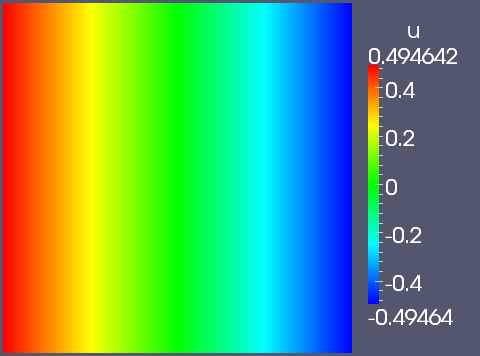
\includegraphics[scale=.425]{figs/aEpsConstant.png}}
\subfigure[$\alpha = 1$]{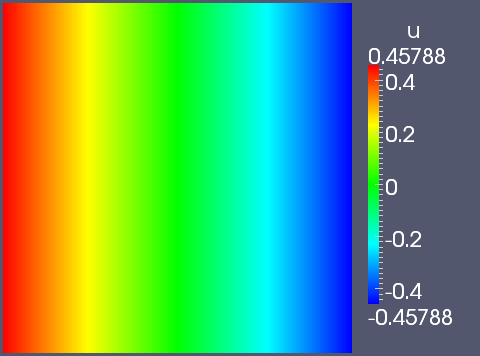
\includegraphics[scale=.425]{figs/aOneConstant.png}}
\caption{Optimal test functions for a $u=1$.}
\end{figure}

\begin{figure}
\centering
\subfigure[$\alpha = \epsilon$]{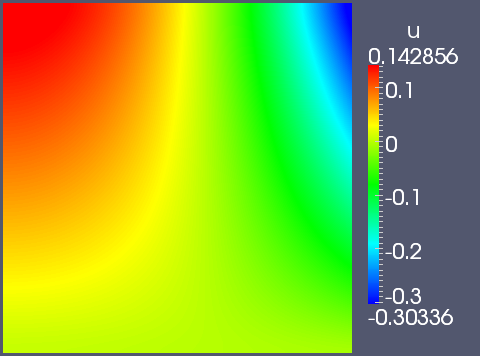
\includegraphics[scale=.425]{figs/aEpsBilinear.png}}
\subfigure[$\alpha = 1$]{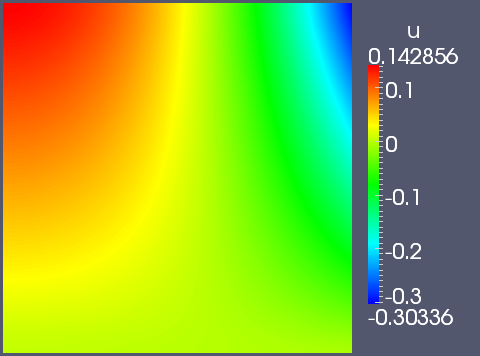
\includegraphics[scale=.425]{figs/aOneBilinear.png}}
\caption{Optimal test functions for a $u=xy$.}
\end{figure}

\begin{figure}
\centering
\subfigure[$\alpha = \epsilon$]{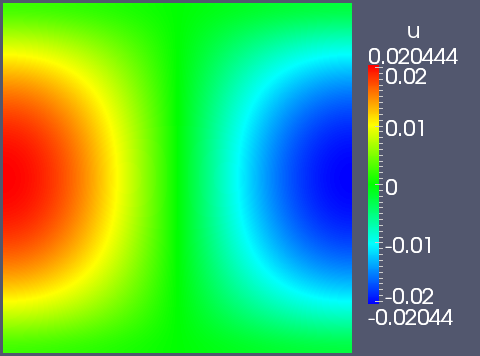
\includegraphics[scale=.425]{figs/aEpsBubble.png}}
\subfigure[$\alpha = 1$]{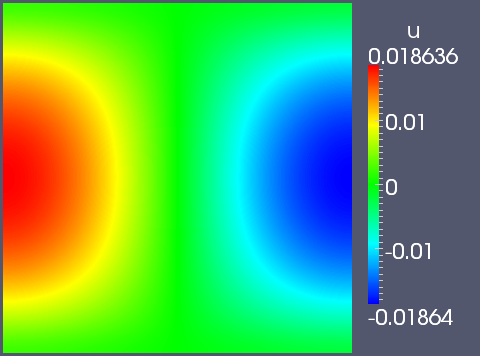
\includegraphics[scale=.425]{figs/aOneBubble.png}}
\caption{Optimal test functions for a $u=x(1-x)y(1-y)$.}
\end{figure}

\begin{figure}
\centering
\subfigure[$\alpha = \epsilon$]{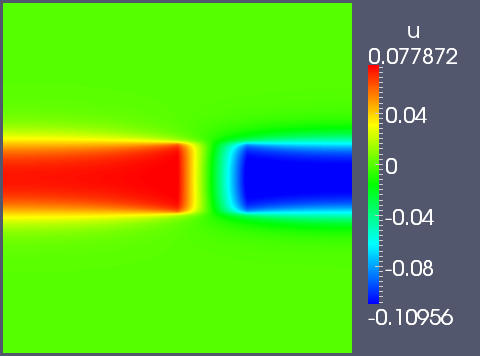
\includegraphics[scale=.425]{figs/aEpsElement.png}}
\subfigure[$\alpha = 1$]{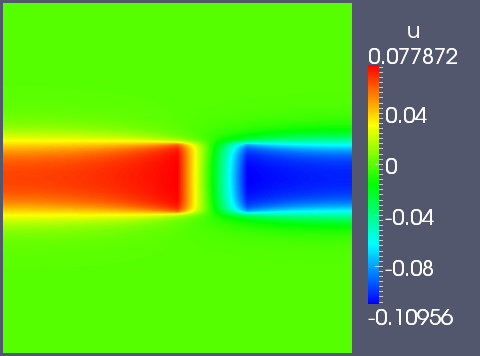
\includegraphics[scale=.425]{figs/aOneElement.png}}
\caption{Optimal test functions for a $u=\left.1\right|_K$, where $K = [.5,.7]\times[.4,.6]$.}
\end{figure}

\section{Test norms for the convection-diffusion equation with first-order term}
\seclab{appendix:timesteppingConfusion}

Very often, the convection-diffusion equation includes a first-order term, such that the form of the equation is
\[
\div\LRp{\beta u - \epsilon \grad u} + \alpha v = f
\]
where $\alpha$ is some constant or function.
%The form of the first order system is 
%\begin{align*}
%\div\LRp{\beta u - \sigma} + \alpha v &= f\\
%\frac{1}{\epsilon}\tau - \grad u &= 0.
%\end{align*}
This first-order term represents a reaction term, modeling production of the solvent $u$.  Most commonly, however, this first order term appears in context of implicit time-stepping methods for the transient convection-diffusion equation
\[
\pd{u}{t}+\div\LRp{\beta u - \epsilon \grad u} = f.
\]
For implicit time-stepping methods, we solve for the solution at the current timestep $u_{t_i} \coloneqq u$ under some approximation of the time derivative: for example, implict Euler uses the first order approximation $\pd{u}{t} \approx \frac{u-u_{t_{i-1}}}{dt}$, introducing a reaction term $u/dt$
\[
\frac{u}{dt}+\div\LRp{\beta u - \epsilon \grad u} = f + \frac{u_{t_{i-1}}}{dt}.
\]
Under this version of the convection-diffusion equation, we modify our test norm to match the magnitude of the first order term $u/dt$
\[
\nor{v,\tau}_V^2 \coloneqq \frac{1}{dt}\nor{v}_{\L}^2 + \nor{\beta\grad v}_{\L}^2 + \epsilon \nor{\grad v}_{\L}^2 + \nor{\tau}_{\L}^2 + \nor{\div \tau}_{\L}^2.
\]
Noting that, according to the previous numerical experiments, the magnitude of the $\L$ term does not appear to create boundary layers in test functions for field variables.  Thus, so long as the $\frac{1}{dt}$ is $O(h)$, the mesh size, we should expect (by a transformation to the unit element) optimal test functions to be locally resolvable using our enriched space.

Recall that proving robustness involves showing energy estimates on the following adjoint equation
\[
\frac{1}{dt}v - \beta\cdot \grad v - \epsilon\del v = u - \epsilon\div \sigma
\]
where $u, \sigma \in \L$ represent functions from the trial space.  
\begin{lemma}
$\frac{1}{dt}\nor{v}_{\L}^2 + \epsilon \nor{\grad v}_{\L}^2 \lesssim \nor{u}_{\L}^2 + \nor{\sigma}_{\L}^2.$
\end{lemma}
\begin{proof}
Multiplying the equation by $v$ and integrating gives
\[
\int \frac{1}{dt} v^2 - \int \beta \cdot \grad v v -  \int \epsilon \del v v = \int u v -  \int \epsilon \div \sigma v.
\]
Integration by parts gives
\[
\frac{1}{dt} \nor{v}^2 + \int \frac{\div \beta}{2} v^2 - \int_\Gamma \frac{\beta_n}{2}v^2 + \epsilon \nor{\grad v}^2 - \epsilon \int_\Gamma v\pd{v}{n}  = \int uv + \int \sigma \epsilon \grad v  - \epsilon \int_\Gamma \sigma_n v
\]
Applying adjoint boundary conditions 
\begin{align*}
v &= 0, \quad \text{on } \Gamma_{\rm out}\\
\pd{v}{n} &= \sigma_n, \quad \text{on } \Gamma_{\rm in}
\end{align*}
reduces this to
\[
\frac{1}{dt} \nor{v}^2 + \int \frac{\div \beta}{2} v^2 + \int_{\Gamma_{\rm in}} \frac{|\beta_n|}{2}v^2 + \epsilon \nor{\grad v}^2 = \int uv + \int \sigma \epsilon \grad v.
\]
An application of Young's inequality on the right hand side completes the proof.  
\end{proof}
If we multiply by $\frac{1}{dt}v$ instead of $v$, we can derive a slightly different bound
\begin{lemma}
$\nor{\frac{1}{dt}v}_{\L}^2 + \frac{\epsilon}{dt} \nor{\grad v}_{\L}^2 \lesssim \nor{u}_{\L}^2 + \nor{\sigma}_{\L}^2$.
\end{lemma}
\begin{proof}
The proof is very similar to the above case. 
\end{proof}

%\section{Conditioning of local matrices}
 

\section{Error propagation in traces}

In \cite{DPGrobustness}, both the graph norm and the constructed test norm (which we refer to as the \textit{robust} test norm) are shown to satisfy the robust bound
\[
\LRp{\nor{u}_{\L}^2 + \nor{\sigma}_{\L}^2 + \epsilon^2\nor{\uh}_{H^{1/2}(\Gh)} + \epsilon\nor{\fnh}_{H^{-1/2}(\Gh)}}^{1/2} \lesssim \nor{\LRp{u,\sigma,\uh,\fnh}}_E
\]
where $\nor{\cdot}_E$ is the energy norm in which DPG is optimal.  The focus of this bound is the $\epsilon$ independence of the $\L$ norms on $u$ and $\sigma$; however, we have not addressed the issue of robustness of the traces $\uh$ and flux $\fnh$ and how it manifests in practice.  

We examine a test problem, with $\Omega = [0,1]^2$.  Inflow conditions\footnote{$u-\epsilon\pd{u}{n}$ approximates $u$ for $\epsilon\ll 1$.  These conditions are set such that we are able to use the robust test norm described in \cite{DPGrobustness2}.} are set such that
\begin{align*}
u \approx u-\epsilon\pd{u}{n} &= 0,\quad x = 0,\quad y \in [0,1],
\end{align*}
and wall boundary conditions are set to mimic a flat plate problem such that
\begin{align*}
%u &= 0,\quad x = 1,\quad y \in [.5,1],\\
u &= 0,\quad y = 0,\quad x \in [.5,1].
\end{align*}
Boundary conditions in the rest of the domain are set such that
\begin{align*}
\pd{u}{n} &= 0,\quad y = 1,\\
\pd{u}{n} &= 0,\quad y = 0,\quad x \in [0,.5].
\end{align*}
We examine the traces along $y=0$.  Recall that traces are discretized as traces of $H^1$-conforming trial functions; thus, whereas we expect convergence in the $\L$ norm for field variables, this is not true for the traces.  In particular, we observe a Gibbs-type phenomena in the propagation of error for traces in Figure~\ref{fig:traceErrors}.  Unlike the field variables, Gibbs-type overshoots and undershoots in the solution are not localized to a single element.  This is due to the increased stencil size for traces, which are not locally supported over one element the way field and flux variables are.
\begin{figure}
\centering
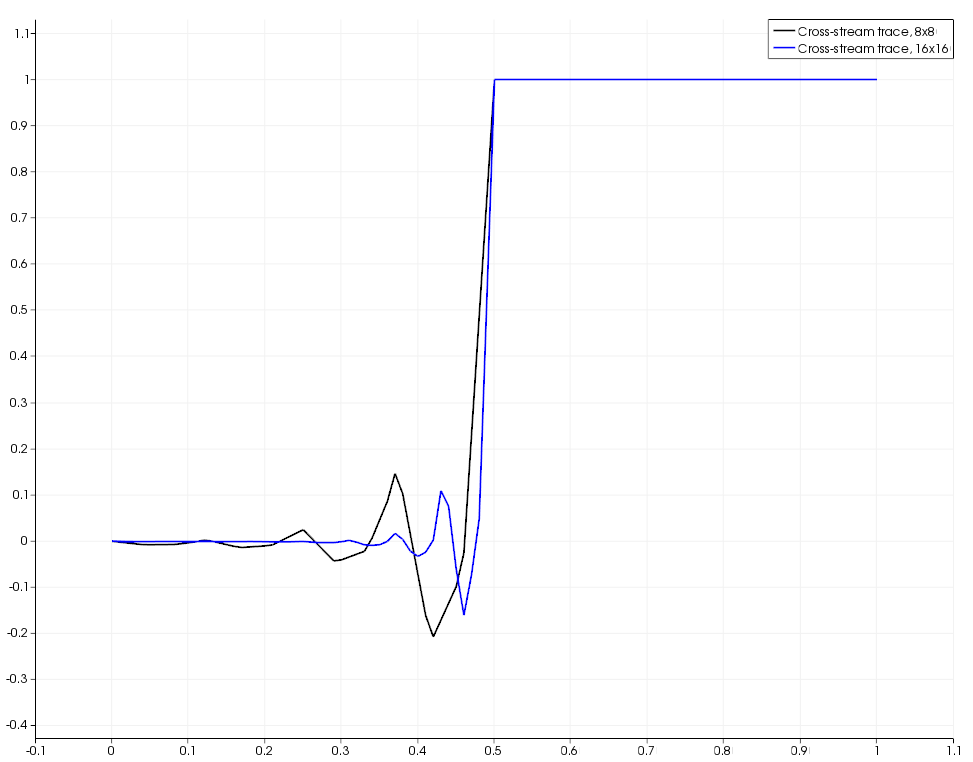
\includegraphics[scale=.4]{figs/CrossTraces.png}
%\subfigure[Cross-stream traces]{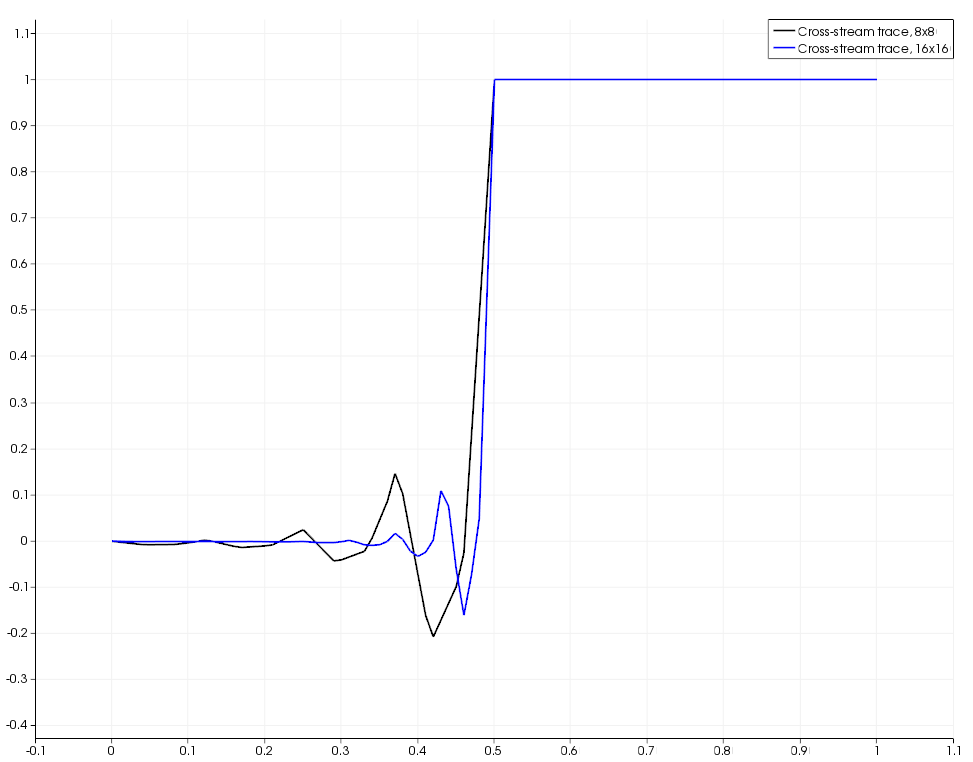
\includegraphics[scale=.3]{figs/CrossTraces.png}}
%\subfigure[Outflow traces]{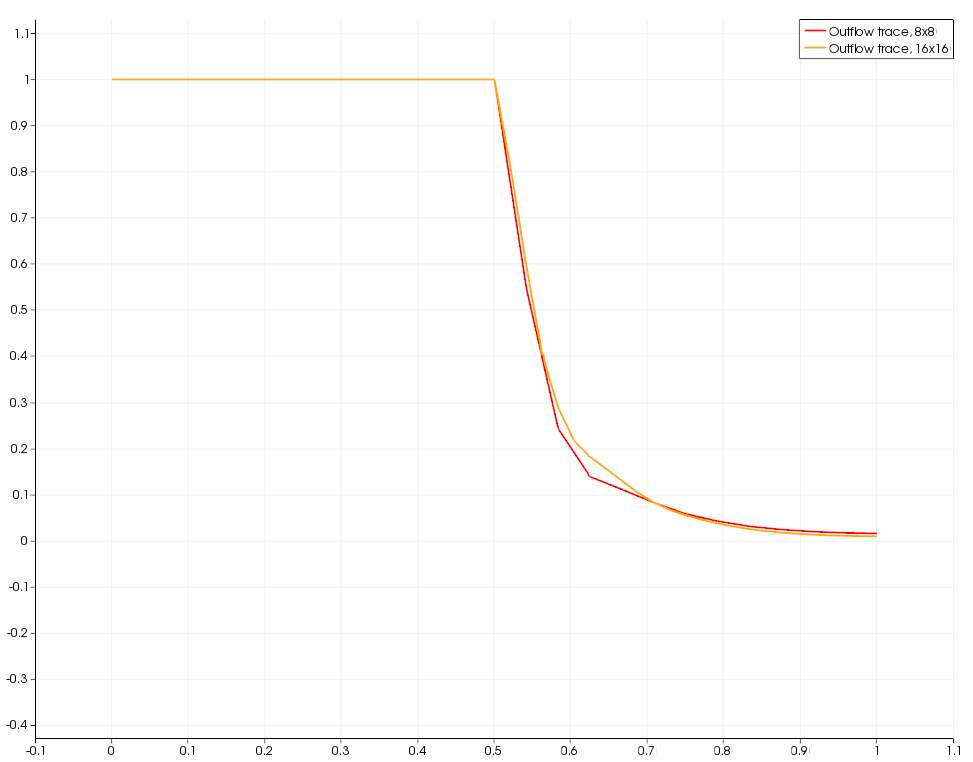
\includegraphics[scale=.3]{figs/OutflowTraces.png}}
%\caption{Difference between outflow and cross-stream traces.}
\caption{$H^1$-type propagation of error along $y = 0$.}
\label{fig:traceErrors}
\end{figure}

\section{Zero-mean scaling}

In \cite{DPGrobustness, DPGrobustness2}, we proved the energy estimate
\[
\nor{v}^2_{\L} \lesssim \nor{u}^2_{\L} + \nor{\sigma}^2_{\L}
\]
which implied that including $\nor{v}$ could be included in the test norm $\nor{v,\tau}_V$ and produce a robust DPG method for convection-diffusion.  However, it is also possible to replace the $\L$ term with the first-order term 
\[
\frac{1}{h^2}\LRb{\int_K v}^2
\]
which is a scaled measure of the average of $v$ over an element.  By H\"{o}lder's inequality, we have that 
\[
\LRb{\int_K v} \leq \LRb{\int_K v^2}^{\frac{1}{2}} \LRb{h^2}^{\frac{1}{2}}, 
\]
implying that 
\[
\frac{1}{h^2}\LRb{\int_K v}^2 \leq \nor{v}^2_{\L}
\]
For the locally conservative version of DPG, we were able to replace $\nor{v}^2_{\L}$ in the test norm with $\frac{1}{h^4}\LRb{\int_K v}^2$, because in context of local conservation (enforced by Lagrange multipliers), elementwise constants are already enforced to be in the test space, so the addition of the mean-squared term to the test norm is solely to enforce a scaling condition enforcing a zero-mean condition on the remainder of the test functions.